%%%%%%%%%%%%%%%%%%%%%%%%%%%%%%%%%%%%%%%%%%%%%%%%%%%%%%%%%%%%%%%%%%%%%%%%%%%%%%%%
%theory.tex: Chapter on light dark matter theory
%%%%%%%%%%%%%%%%%%%%%%%%%%%%%%%%%%%%%%%%%%%%%%%%%%%%%%%%%%%%%%%%%%%%%%%%%%%%%%%%
\chapter{Theoretical Framework}
\label{theory}
%%%%%%%%%%%%%%%%%%%%%%%%%%%%%%%%%%%%%%%%%%%%%%%%%%%%%%%%%%%%%%%%%%%%%%%%%%%%%%%%
There are two key aspects to the theory used in the search presented here: a model of a new physics which could produce dark matter used to simulate its interactions and determine our sensitivity, and a model of known physics, necessary to understand conventional processes which could mimic dark matter interactions as well as describe the initial states produced in the collision and the response of the detector to any produced particles.

The primary framework used to describe currently known particle physics is the standard model (SM), a quantum field theory which describes the set of known fundamental particles and their interactions.
In classical theories, particle interactions can be described via forces proportional to fields, such as the electromagentic field applying a force directly proportional to the charge of a given particle.
In quantum field theories, particle interactions are instead described through the exchange of a gauge boson, allowing them to satisfy the requirements of special relativity and quantum physics. 
The SM contains five gauge bosons, which describe interactions with the nuclear strong, electroweak, and Higgs fields.
In addition, the SM includes six quarks, colored particles which can interact via the strong force, and six leptons, particles which only interact via the electroweak force.
A graphical representation of these fundamental particles is shown in \Cref{fig:SM}, along with numerical values of some of their physical properties.

\begin{figure}
	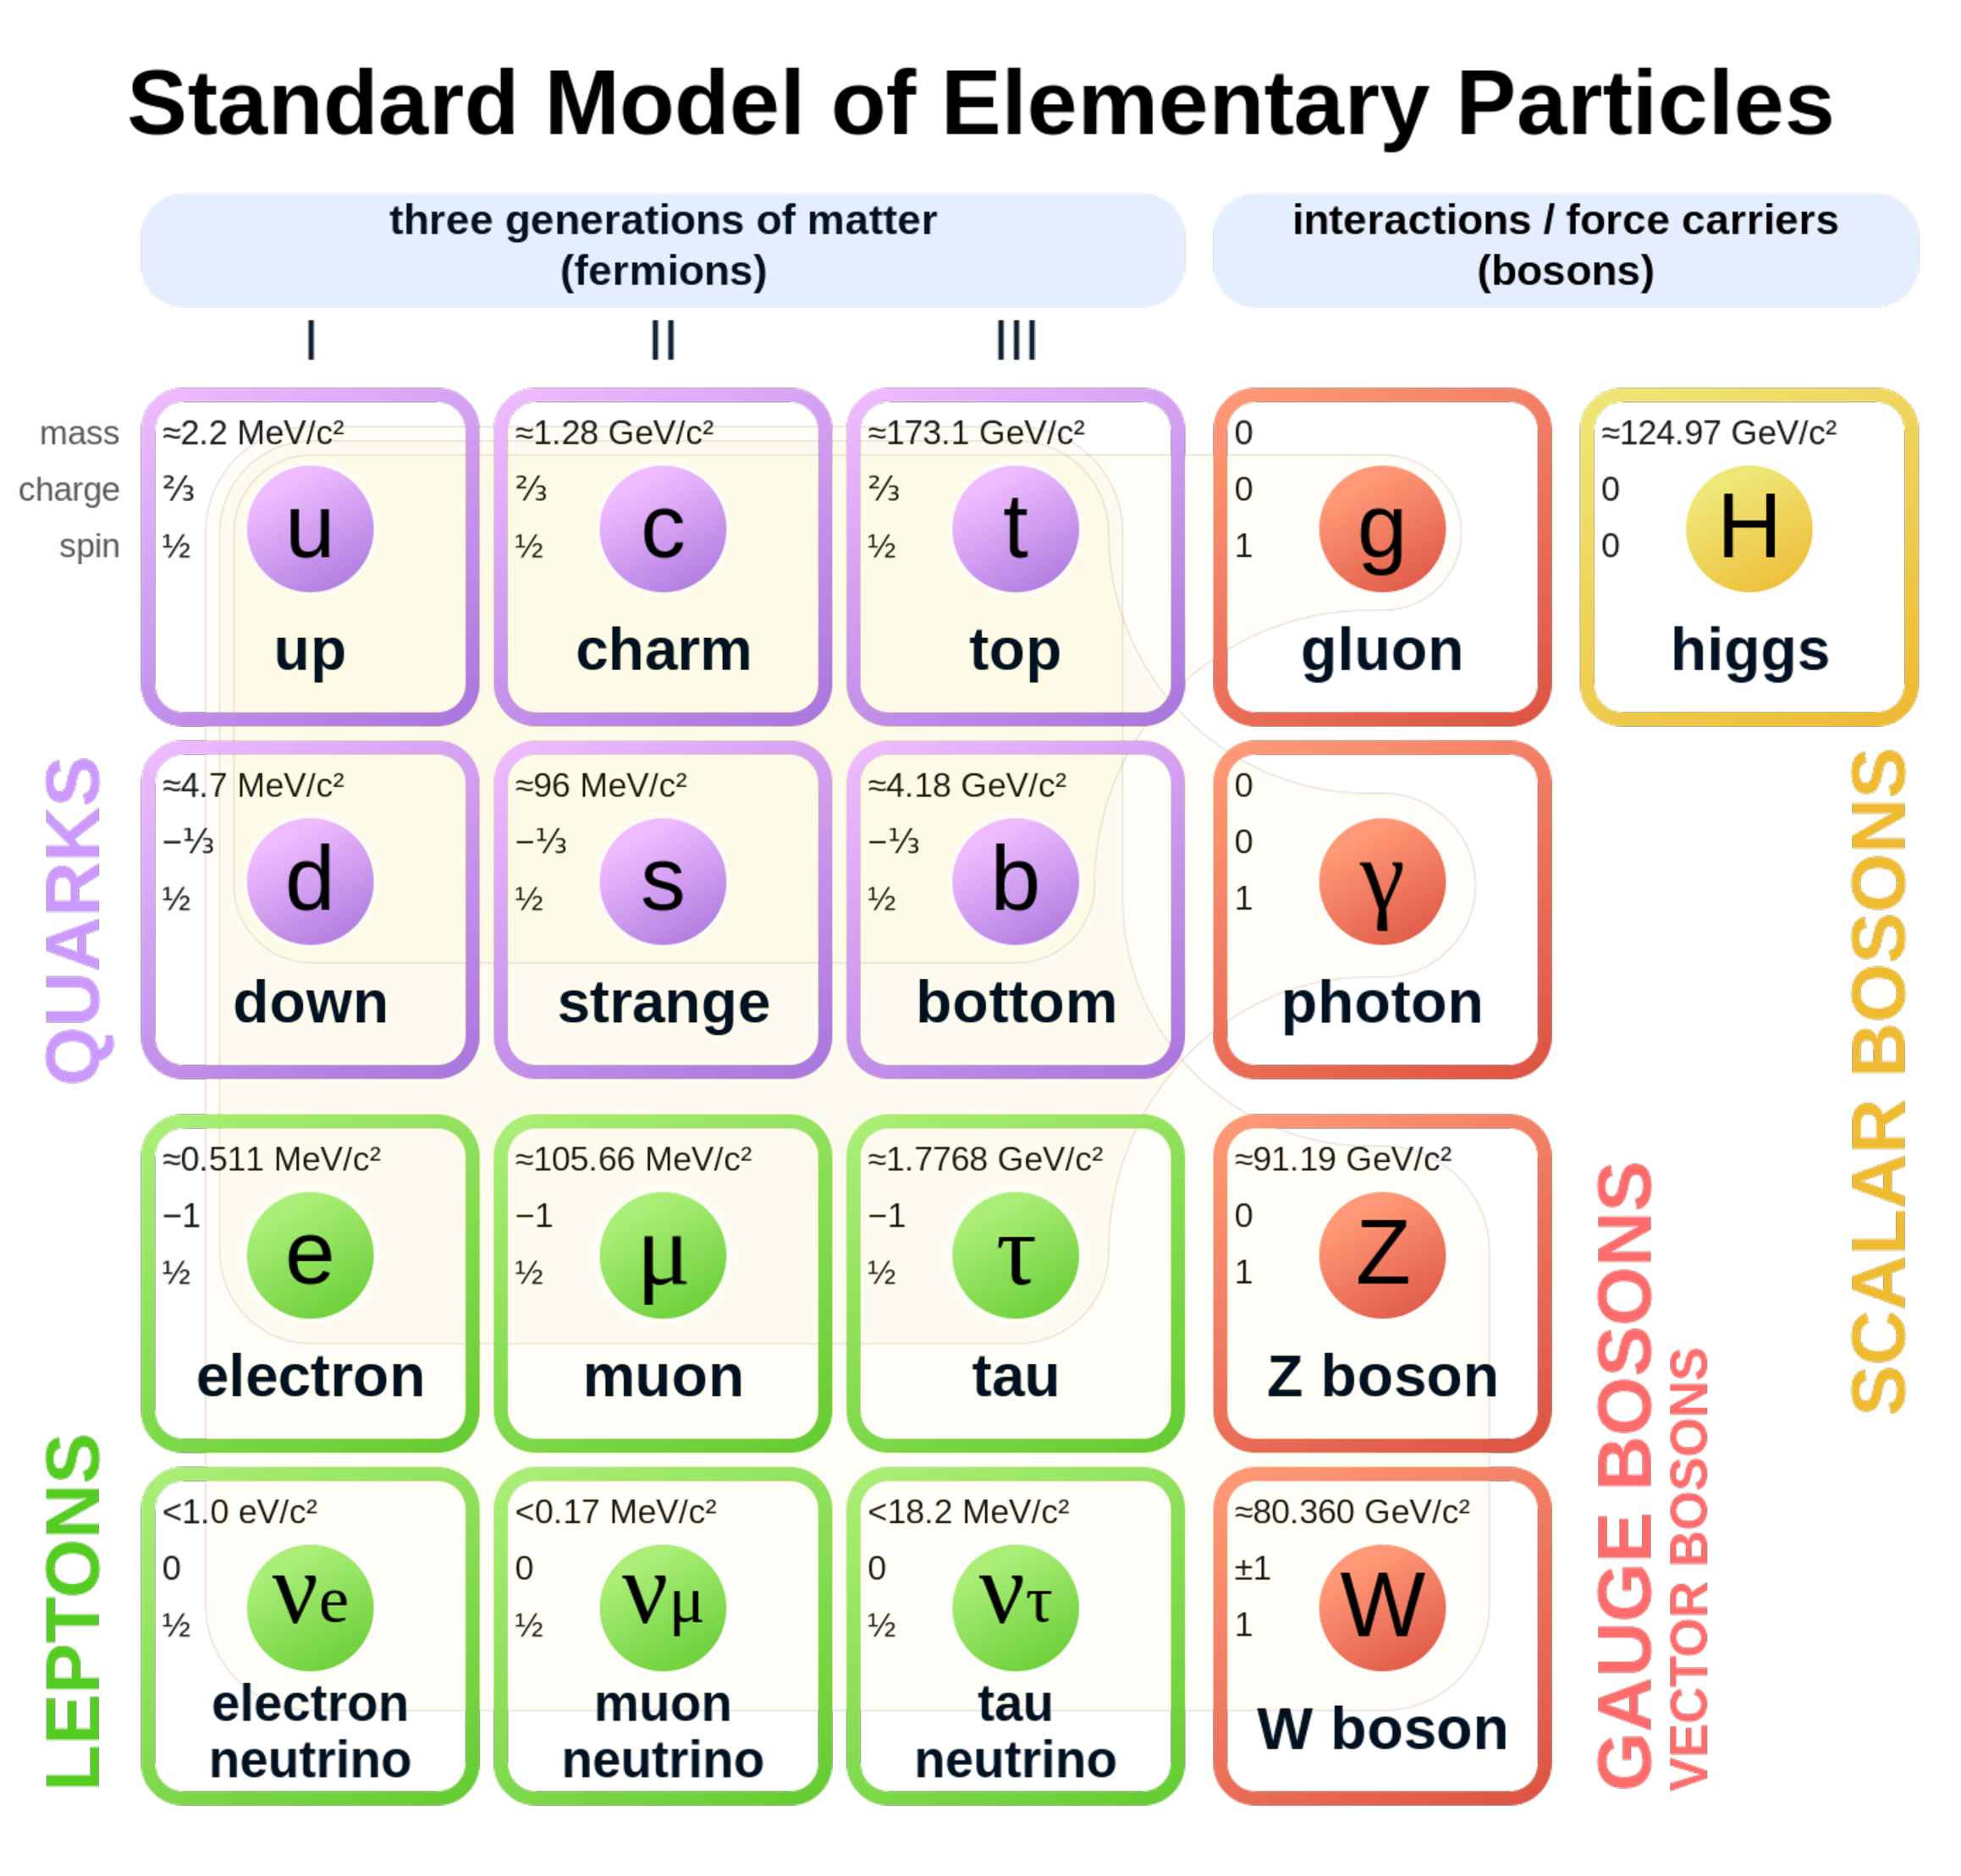
\includegraphics[width=0.9\textwidth]{figures/smParticles.pdf}
	\centering
	\caption{Fundamental particles within the standard model.}
	\label{fig:SM}
\end{figure}

Developed over several decades through close collaboration between theory and experiment, the SM has been extremely successful at predicting a wide range of observed physics phenomena to date (FIND SM VALIDATION).
Despite this success, there are several missing pieces in the SM such as gravity, neutrino masses, dark energy, and most significant to this paper, dark matter.
While these phenomena are observed in experiments, the lack of full information about the nature of the particles themselves or their interaction prevent their inclusion in the SM, and so keep it from being a complete description of all observed particle interactions.  

\section{Thermal Dark Matter}
To help identify dark matter signatures that may be visible in a detector based experiment, several assumptions can be made relating to its nature. 
The primary one made here is that of thermal dark matter.
The core assumption of thermal dark matter models is that the interaction between dark matter and SM matter is significant enough that for some period of time in the early universe dark matter is in thermal equilibrium with standard model matter.
This allows dark matter to be produced simultaneously with SM matter during the universes' inception rather than as a separate process, and also requires that dark matter have some coupling to SM matter, which would also be necessary for its observation in an experiment like CMS.

This thermal equilibrium is achieved to due the high temperature and density of the early universe, where despite small SM couplings dark matter particles can be frequently produced through interactions with standard model particles and produce standard model particles through their own interactions and decays.
As the universe expands and cools, the rate of these interactions decreases until the dark matter interaction rate fall below the Hubble expansion rate and "freezes out", leaving thermal equilibrium with SM matter and leaving its phase-space distribution subject only to the universe expansion and eventual structure formation \cite{thermalDM}.

For any given thermal dark matter model a 'relic target' cross section can be calculated - the cross section required to produce the density of dark matter seen today.
For any given cross section, the thermal relic model will set a specific freeze-out temperature and number density.
By combining this number density with the observed astronomical mass density, the thermal relic cross section can be related directly to a dark matter mass, with heavier particles requiring lower number densities and therefore later freeze-out temperatures and larger interaction cross sections.

\section{Light Dark Matter}
Traditional searches for thermal dark matter have tended to focus on models which interact via the nuclear weak force, which have relatively larger dark matter mass requirements (M$>~few GeV$), and so are easier to observe with indirect detection experiments searching for collisions of halo dark matter particles with passive detectors.
While this larger mass, weakly interacting phase space is well covered from a wide variety of experments, dark matter could also be explained using mediators in a 'light' mass region, ~MeV to ~GeV, which act as a 'portal' to couple dark sector particles to the SM \cite{darkSectors}.


A potential renormalizable interaction which can be introduced to the SM which could create this light coupling is a kinetic mixing between a new gauge boson with field strength $F'_{\mu\nu}$ and the hypercharge field $B^{\mu\nu}$ through the operator $\mathcal{L}$ (\Cref{eq:LDMlagrangian}). 

\begin{equation}
	\label{eq:LDMlagrangian}
	\mathcal{L} = - frac{\epsilon}{2} B^{\mu\nu}F'_{\mu\nu}
\end{equation}

For small mixing paramater $\epsilon$ and light gauge bosons, these new couplings align with those of the SM photon \cite{Bauer_2018} and so this new gauge boson is referred to as the "dark photon", or A'.
Through these couplings, any SM process which produces a photon could instead produce a dark photon, with suppression proportional to the mixing parameter.

This coupling represents the minimal kinetic mixing, encoding the kinetic coupling as a free parameter instead of arising from specific interactions within a chosen theory. 
While technically forming a dark sector on its own, this model must be extended with additional particles to act as dark matter candidates, as models with only dark photons would cause them to decay back into SM particles.
These dark matter candidates would couple to the dark photon via dark-sector gauge interactions with some coupling strength $g_D$, and can be either fermions or scalar bosons.
As these dark sector particles are assumed to be invisible to our detector, the nature of these dark sector particles is only seen through the branching fraction of the dark photon decaying to SM particles or dark matter particles.
As this search focuses on invisible dark photon signatures, it is assumed that $g_D$ is much larger than $\epsilon$ and that the mass of the dark matter candidates is less than twice the A' mass such that they will decay dominantly to dark matter particles and have a branching fraction to invisible near one.

\section{Targeting Dark Matter Production}
If a light dark matter coupling were present, there are several potential signatures that could appear in an experiment like CMS.
Traditional searches in CMS look for particle production in the initial scattering process between proton constituents.
As a light dark matter coupling would allow mixing between the \aprime and any standard model photon, dark matter could be produced in initial state collisions with electromagnetic interactions between partons that produce photons that then mix with the \aprime.

Unfortunately, decays of the \aprime outside of the detector or into other dark matter particles which are invisible to CMS make this initial production mode very difficult to distinguish.
Events with large initial state radiation from the partons can make this signal visible as a large missing transverse momentum in the event, but the large reduction in acceptance from this type of requirement causes the resulting limit to be very weak.

Instead of searching for dark matter production in the initial state, the signal could appear in a secondary interaction between a final state particle and the detector itself.
The relatively small masses of light dark matter particles limits the loss in the interaction rate due to the much lower center of mass energy in these secondary interactions compared to the initial collision, and the high particle flux and large size of the detector result in a significant fixed target luminosity.

The primary signature of a secondary interactions between a particle emitted from the initial collision and the detector would be missing energy carried by the invisible \aprime and a change in the trajectory of the visible particle.
These types of signatures are difficult to observe in particles with have large standard model interaction rates, as the shower of particles produced in their interactions can lead to large uncertainties in their energy measurement and little hope of observing trajectory differences.
In addition, high interaction rates expose particles to less of the detector as they are stopped relatively quickly, reducing the effective luminosity.

For these reasons, the selections in this search target potential dark matter interactions of final state muons.
As muons have small standard model cross sections they lose very little energy while they traverse the detector, leading to high consistency in projecting their trajectory and observing potential changes, as well as low rates of stopped muons due to standard model processes which could fake the energy loss to an \aprime.

With a light dark matter mixing, muons would primarily produce dark matter in the mass ranges of interest via a process known as \dbrem, where a dark matter particle is emitted from a muon as it recoils from the electromagnetic field of a nucleus in the detector (\Cref{fig:dbrem_feyn}).
While other processes, such as photoproduction of vector mesons which then decay invisibly through dark matter coupling, would also be present with the assumed coupling, only \dbrem is considered in this search due to its significantly larger production rate.

\begin{figure}[ht]
	\centering
	\label{fig:dbrem_feyn}
	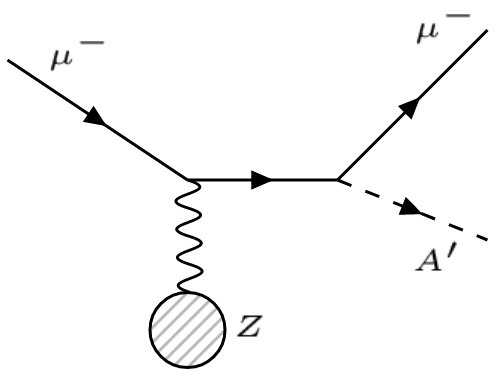
\includegraphics[width=\textwidth]{figures/dbrem_feyn_diagram.jpg}
        \caption[Dark Bremmstrahlung Feynman Diagram]{Dark Bremsstrahlung caused by a muon interacting with a nucleus with atomic number Z.}
\end{figure}

As an additional feature of muon-initiated \dbrem, results from this search are also sensitive to dark matter models which replace the generic dark matter mixing with an asymmetric coupling to the lepton generations.
While lepton universality is built into the standard model, no such requirement is necessary for new physics models. 
Instead of the fully generic kinetic mixing presented in \Cref{eq:LDMlagrangian}, the dark photon gauge field can be chosen to contain an additional current which carries charge proportional to muon number minus tau number, ($L_\mu - L_\tau$) \cite{neut_trident}.
This type of field would result in a dark matter coupling that preferentially interacts with muons and tauons, and has few existing constraints as it only would affect neutrinos and unstable leptons.

There are several experimental anomalies which could potentially be explained by an asymmetric lepton coupling of this type.
The measurement of the muon magnetic moment by the Fermilab E989 experiment \cite{gminus2}, combined with the original result from Brookhaven \cite{gminus2_bnl} leads to a 4.2 $\sigma$ discrepancy with the theoretical prediction \cite{gminus2_theory}. 
This could potentially be explained by a dark matter signal which preferentially couples to muons, as the dark matter coupling would alter the muon magnetic moment through additional loop diagrams.
A muon-philic cross section would also have a larger thermal relic cross section, as requiring a muon or tau coupling in its production reduces the available paths in its creation and so requires increasing the remaining cross section to achieve the same freeze-out number density.

\section{Z-Bosons and the DY Process}


%%%%%%%%%%%%%%%%%%%%%%%%%%%%%%%%%%%%%%%%%%%%%%%%%%%%%%%%%%%%%%%%%%%%%%%%%%%%%%%%
